\documentclass[11pt,a4paper]{article}

\usepackage[margin=1in]{geometry}
\usepackage{amsmath,amssymb,amsthm,mathtools}
\usepackage{stmaryrd}
\usepackage{booktabs}
\usepackage{enumitem}
\usepackage{hyperref}
\usepackage[capitalize]{cleveref}
\usepackage{tikz}
\usetikzlibrary{arrows.meta,calc,positioning,shapes.geometric}

\hypersetup{
  colorlinks=true,
  linkcolor=blue,
  citecolor=blue,
  urlcolor=blue,
  pdfauthor={Christopher Albert},
  pdftitle={Conditioning by Fibers: A Chain-Rule Semantics for Probability, Many-Valued Logic, and Impossible Evidence}
}

\emergencystretch=3em

\newtheorem{theorem}{Theorem}[section]
\newtheorem{lemma}[theorem]{Lemma}
\newtheorem{proposition}[theorem]{Proposition}
\newtheorem{corollary}[theorem]{Corollary}
\newtheorem{definition}[theorem]{Definition}
\newtheorem{example}[theorem]{Example}
\newtheorem{remark}[theorem]{Remark}

\newcommand{\cred}{\mathsf{cred}}
\newcommand{\Cond}{\mathsf{Cond}}
\newcommand{\Adm}{\mathsf{Adm}}
\newcommand{\Sol}{\mathsf{Sol}}
\newcommand{\collapse}{\kappa}
\newcommand{\negc}{\mathord{\sim}}
\newcommand{\conjc}{\otimes}
\newcommand{\disjc}{\sqcup}
\newcommand{\half}{\tfrac12}
\newcommand{\quarter}{\tfrac14}
\newcommand{\three}{\mathbf{3}}
\newcommand{\Real}{\mathbb{R}}
\newcommand{\val}[1]{\llbracket #1 \rrbracket}
\newcommand{\Lean}[1]{\texttt{#1}}
\newcommand{\seq}{\vdash}

\title{Conditioning by Fibers:\\
\large A Chain-Rule Semantics for Probability, Many-Valued Logic, and
Impossible Evidence}
\author{Christopher Albert\\
\small Institute for Theoretical and Computational Physics\\
\small Graz University of Technology}
\date{June 2026}

\begin{document}

\maketitle

\begin{center}
\small
Transparenzhinweis: Mit Unterstützung von Claude- und GPT-Modellen erstellt; Inhalt, Auswahl und fachliche Prüfung verantwortet der Autor.
\end{center}

\begin{abstract}
This paper isolates a small formal core for reasoning with impossible
evidence.  Values usually live in $[0,1]$ with complement
$\negc c=1-c$, product conjunction $a\conjc b=ab$, and De Morgan
disjunction $a\disjc b=a+b-ab$.  The primitive conditional object is
the admissibility judgment
\[
  \Adm(c;j,e)\quad\Longleftrightarrow\quad c e=j.
\]
The displayed set
\[
  \Cond(j,e)=\{c\in[0,1]:ce=j\}
\]
is the external fiber of that relation.  It is a singleton $\{j/e\}$
when $e>0$ and $j\le e$; it is all of $[0,1]$ when $j=e=0$; it is
empty when $j>e$.  Impossible evidence therefore does not imply
everything.  It imposes no equation.

The paper proves three consequences of that small observation.  First,
the product De Morgan triplet collapses to the Kleene lattice
$\{0,\half,1\}$, and the collapse matches LP consequence with
positivity on $[0,1]$, and K$_3$ consequence with certainty.  Second,
that bridge cannot be extended to conditioning: no truth function on
$\{0,\half,1\}$ reproduces min-copula conditioning after collapse.
Third, adding a total internal conditional with modus ponens,
conditional proof, and contraction is impossible; the product residuum
is forced at positive antecedents and violates contraction.  Liar and
Russell equations become solution sets rather than detonators:
$c=1-c$ has the unique solution $\half$, while the truth-teller has
the same shape as zero-evidence conditioning, the whole interval.

The useful contribution is the separation principle: truth values,
dependence data, and conditional inference are distinct inputs.  The
same fiber construction works on the continuum, on the Boolean carrier,
and on three-valued variants once the carrier and conjunction are
fixed.  A non-singleton fiber is propagated: subsequent rules carry the
admissible values instead of selecting a quotient at zero evidence.
Unknown dependence is handled the same way: with the joint confined to
its Fr\'echet interval, the conditional propagates as an interval that
is either robust or dependence-sensitive against a threshold.  Finite
toy models give a first formalized cut at a foundation: dependence
contexts, proof provenance, hypothetical branches without explosion, a
generative connective calculus, and the $\sqrt2$ number-theoretic seed.
The formal results are machine-checked in Lean 4 with Mathlib; theorem
names are cited in the text.
\end{abstract}

\tableofcontents

\section{Contribution Hierarchy}

The paper keeps one mechanism and the obstructions around it.  Adjacent
developments are useful only when they support that mechanism.

\begin{table}[h]
\centering
\begin{tabular}{@{}p{0.08\linewidth}p{0.29\linewidth}p{0.50\linewidth}@{}}
\toprule
Rank & Component & Reason \\
\midrule
1 & Chain-rule conditioning as an admissibility judgment &
It gives the uniform object: the fiber of $c\conjc e=j$.  At positive
coherent evidence it is ordinary division; at zero evidence it is
non-explosive: $\Cond(0,0)=[0,1]$. \\
2 & Collapse and LP/K$_3$ bridge &
It explains why the same real-valued semantics has a paraconsistent
reading at positivity and a paracomplete reading at certainty. \\
3 & No truth-functional conditional bridge &
It is a finite obstruction, not a philosophical preference: two
interior pairs force two different outputs for the same collapsed
input $(\half,\half)$. \\
4 & Curry block &
It explains why conditioning must stay external.  A total internal
arrow with modus ponens, conditional proof, and contraction cannot
exist on this carrier. \\
5 & Solution sets for self-reference &
It gives a compact foundations payoff: paradoxes become equations
with solution sets. \\
\midrule
Scope boundary & Arithmetic coding, bootstrapping analogies, graded numerical analysis &
They do not support the central theorem package.  They need separate
venues and separate motivation. \\
\bottomrule
\end{tabular}
\caption{Claim hierarchy.  The paper keeps the formal core and separates
adjacent material unless it supports the same theorem package.}
\label{tab:claims}
\end{table}

The resulting submission has one thesis:

\[
\boxed{
\text{inference constrains admissible values; impossible evidence
constrains none.}}
\]

That thesis is elementary.  Its force comes from the surrounding
no-go results.

The title phrase \emph{conditioning by fibers} is literal.  Fix the
evidence value $e$.  Multiplication by $e$, or the chosen conjunction
with $e$, is a map from candidate conditionals to joint values.  A
conditional is admissible exactly when it lies in the preimage of the
given joint value.  At positive coherent evidence, probability theory
has a singleton fiber and writes a quotient.  Boolean and many-valued
variants restrict the carrier; the same preimage construction still
applies.  A truth table would have to choose one value.  The singular
fiber at zero evidence is a set of admissible values.  Logical
consequence is the same inclusion read over valuations rather than
values; one operator covers both, and a later section makes it explicit.

\section{The Setting}

\subsection{Values and Operations}

\begin{definition}[Credence value]
A credence is a real number $c\in[0,1]$.
\end{definition}

The basic operations are
\[
  \negc c=1-c,\qquad
  a\conjc b=ab,\qquad
  a\disjc b=\negc(\negc a\conjc\negc b)=a+b-ab.
\]
The product is the product t-norm; the disjunction is its De Morgan
dual.  These operations are standard in many-valued and fuzzy logic
\cite{zadeh1965,goguen1969,hajek1998,klement2000,cintula2011}.
They are also familiar probabilistic expressions: if $A$ and $B$ are
independent, then
\[
  P(A\cap B)=P(A)P(B),\qquad
  P(A\cup B)=P(A)+P(B)-P(A)P(B).
\]
The paper never assumes independence by default.  The product
$a\conjc b$ is an algebraic operation on values.  A joint credence
$j=\cred(A\land B)$ is separate data.

\begin{figure}[h]
\centering
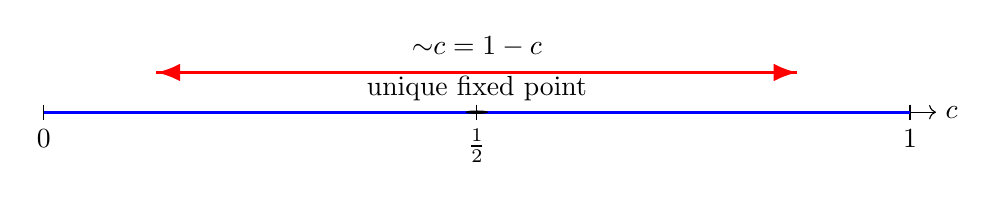
\begin{tikzpicture}[x=11cm,y=1.2cm]
  \draw[->] (0,0) -- (1.03,0) node[right] {$c$};
  \draw (0,0.08) -- (0,-0.08) node[below] {$0$};
  \draw (0.5,0.08) -- (0.5,-0.08) node[below] {$\half$};
  \draw (1,0.08) -- (1,-0.08) node[below] {$1$};
  \draw[very thick,blue] (0,0) -- (1,0);
  \draw[very thick,red,-{Latex[length=3mm]}] (0.13,0.42) -- (0.87,0.42);
  \draw[very thick,red,-{Latex[length=3mm]}] (0.87,0.42) -- (0.13,0.42);
  \node[above] at (0.5,0.48) {$\negc c=1-c$};
  \draw[fill=black] (0.5,0) circle (0.012);
  \node[above] at (0.5,0.02) {unique fixed point};
\end{tikzpicture}
\caption{The complement reverses the unit interval and fixes only
$\half$.  Lean: \Lean{Cred.Credence.neg\_fixed\_point\_unique}.}
\label{fig:unit-interval}
\end{figure}

The verified algebraic facts are routine but important:
\[
\begin{gathered}
\negc\negc c=c,\quad
a\conjc b=b\conjc a,\quad
(a\conjc b)\conjc c=a\conjc(b\conjc c),\\
a\conjc 1=a,\quad a\conjc 0=0,\quad
\negc(a\conjc b)=\negc a\disjc\negc b.
\end{gathered}
\]
Conjunction is idempotent only at the Boolean boundary:
\[
  c\conjc c=c \quad\Longleftrightarrow\quad c\in\{0,1\}.
\]
Lean: \Lean{Cred.Credence.conj\_idempotent\_iff}.  Thus intermediate
credences are not hidden truth values.

\subsection{Algebraic Form}

The construction is carrier-independent.  Let $V$ be a value carrier
with a conjunction-like operation $\conjc$, bottom $0$, and top $1$.
Given evidence $e\in V$ and joint value $j\in V$, define the primitive
admissibility judgment
\[
  \Adm_V(c;j,e)\quad:\Longleftrightarrow\quad c\conjc e=j.
\]
This judgment needs equality and conjunction.  It does not need sets.
After the surrounding mathematics has predicates or sets, one may
write the fiber.  For fixed evidence $e$, put
\[
  m_e(c)=c\conjc e.
\]
Then
\[
  \Cond_V(j,e)=\{c\in V:\Adm_V(c;j,e)\}=m_e^{-1}(j).
\]
The word fiber is used only in this ordinary mathematical sense:
preimage under the multiplication-by-$e$ map.  The paper uses this set
notation as metalanguage.

For the Boolean carrier $\mathbf 2=\{0,1\}$ with $\conjc=\wedge$:
\[
  \Cond_{\mathbf 2}(j,1)=\{j\},\qquad
  \Cond_{\mathbf 2}(0,0)=\{0,1\},\qquad
  \Cond_{\mathbf 2}(1,0)=\varnothing.
\]
Classical conditioning on true fixes the value.  Conditioning on
false leaves the conditional unconstrained unless the joint value is
impossible.

For the Kleene carrier $\three=\{0,\half,1\}$, the same schema applies
with the chosen three-valued conjunction:
\[
  \Cond_{\three}(j,e)=\{c\in\three:c\wedge e=j\}
\]
for the usual strong-Kleene/Godel conjunction $\wedge=\min$.
There is a closure caveat.  The literal set
$\{0,\half,1\}\subset[0,1]$ is not closed under product, since
$\half\cdot\half=\quarter$.  A three-valued product reading is
therefore a quotient of the continuum, while an internal three-valued
logic uses its own closed conjunction, usually $\min$.

\subsection{Conditioning as a Relation}

Conditional probability is usually introduced by division:
\[
  P(A\mid B)=\frac{P(A\land B)}{P(B)},\qquad P(B)>0.
\]
H\'ajek argues that this ratio is not a general analysis of
conditional probability \cite{hajek2003conditional}.  R\'enyi and
Popper instead treat conditional probability as primitive
\cite{renyi1955,popper1959,krauss1968,dubins1975}.  De Finetti's
conditional-event tradition makes the same point in a betting idiom:
if the antecedent fails, the bet is void rather than true
\cite{definetti1936,egre2020part1,egre2021}.  Current work on
indicative conditionals still turns on this boundary between truth,
probability, and undefinedness \cite{egre2025}.

Here the primitive is the chain rule alone:
\[
  \cred(A\mid B)\,\cred(B)=\cred(A\land B).
\]
Given joint value $j$ and evidence value $e$, define
\[
  \Adm(c;j,e)\quad:\Longleftrightarrow\quad c e=j.
\]
The associated fiber is
\[
  \Cond(j,e)=\{c\in[0,1]:c e=j\}.
\]
This is the weak-definition move: keep the identity that survives the
singular case, rather than the quotient that requires $e>0$.  The
analogy stops at uniqueness.  At $e=j=0$, the fiber is genuinely
underdetermined.

\begin{theorem}[Admissible-set trichotomy]
\label{thm:trichotomy}
For $j,e\in[0,1]$:
\[
\Cond(j,e)=
\begin{cases}
\{j/e\}, & e>0\ \text{and}\ j\le e,\\[2mm]
[0,1], & e=0,\ j=0,\\[1mm]
\varnothing, & j>e.
\end{cases}
\]
\end{theorem}

\noindent
Lean:
\Lean{Cred.Credence.cond\_singleton\_of\_pos},
\Lean{Cred.Credence.cond\_zero\_zero\_univ},
\Lean{Cred.Credence.cond\_nonempty\_iff}.

\begin{proof}
If $e>0$, the equation $ce=j$ has the unique solution $c=j/e$.
Since $c\le1$, existence requires $j\le e$.
If $e=0$, the equation is $0=j$.  For $j=0$ every $c$ solves it.
For $j>0$ none does.  The last case is included in $j>e$.
\end{proof}

When the fiber is not a singleton, later reasoning need not stop.
The next step carries the set of admissible values.  A positive
evidence step carries a singleton and therefore behaves like ordinary
Bayes division.  A zero-evidence step carries the whole interval.  A
downstream rule then maps that interval, intersects it with new
constraints, or leaves it unchanged.  This is the same discipline used
by interval and credal-set methods: compute with the set until extra
structure selects a value.  Here the set is the fiber of the
chain-rule equation itself, not a prior ignorance model.
The price is explicit: conditioning is no longer a total function at
singular evidence.  Later rules must carry sets of possible values.
This bookkeeping is the mechanism.  It replaces division by zero and
ex falso with propagation of the remaining admissible values.

\begin{figure}[h]
\centering
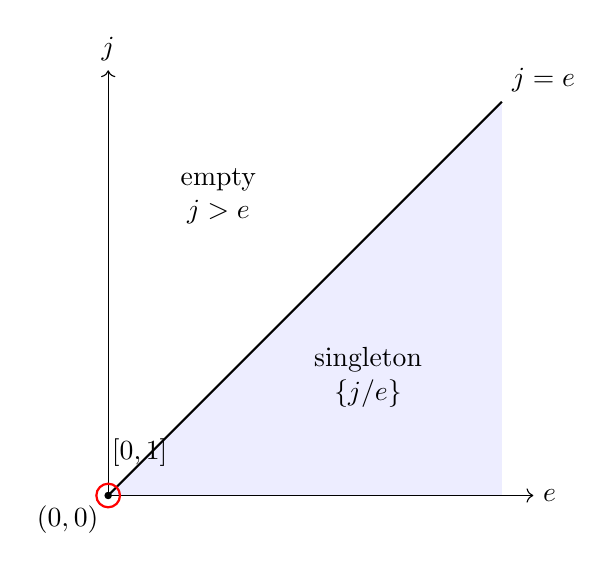
\begin{tikzpicture}[scale=5]
  \fill[blue!7] (0,0) -- (1,0) -- (1,1) -- cycle;
  \draw[->] (0,0) -- (1.08,0) node[right] {$e$};
  \draw[->] (0,0) -- (0,1.08) node[above] {$j$};
  \draw[thick] (0,0) -- (1,1) node[above right] {$j=e$};
  \draw[fill=black] (0,0) circle (0.008);
  \node[below left] at (0,0) {$(0,0)$};
  \node[align=center] at (0.66,0.30) {singleton\\$\{j/e\}$};
  \node[align=center] at (0.28,0.76) {empty\\$j>e$};
  \node[align=left] at (0.08,0.11) {$[0,1]$};
  \draw[thick,red] (0,0) circle (0.03);
\end{tikzpicture}
\caption{The chain rule as geometry.  The coherent region is
$j\le e$.  Positive evidence gives a point.  The origin gives the
whole vertical fiber of possible conditionals.}
\label{fig:cond-geometry}
\end{figure}

This is the whole non-explosion mechanism.  From impossible evidence
one obtains no arbitrary conclusion because no conclusion is selected.
The equation has lost rank.

\section{Binary and Continuous Cred}
\label{sec:binary-continuous}

Write $c$ for the value of ``$A$ given $B$'', $e$ for the value of $B$,
and $j$ for the value of ``$A$ and $B$''.  The basic relation is
$ce=j$.  Reading it on the Boolean carrier and on $[0,1]$ separates two
ideas that ordinary conditional probability folds together: loss of
constraint at impossible evidence, and freedom in the joint.

\subsection{Binary}
On $\mathbf 2=\{0,1\}$ the joint is Boolean conjunction $j=A\land B$,
fixed by the two truth values.  With $e=B$ the equation $ce=j$ gives:
\begin{itemize}[nosep]
\item $B=1$: then $c\cdot1=j=A$, so $c=A$.
\item $B=0$: then $c\cdot0=0$ holds for $c=0$ and $c=1$, so $c$ is
unconstrained.
\end{itemize}
\begin{center}
\begin{tabular}{@{}cccc@{}}
\toprule
$A$ & $B=e$ & $j=A\land B$ & admissible $c=(A\mid B)$\\
\midrule
$0$ & $0$ & $0$ & $0$ or $1$\\
$1$ & $0$ & $0$ & $0$ or $1$\\
$0$ & $1$ & $0$ & $0$\\
$1$ & $1$ & $1$ & $1$\\
\bottomrule
\end{tabular}
\end{center}
True evidence fixes the conditional to the value of $A$; false evidence
leaves it free.  This is the binary form of no ex falso.  The Boolean
carrier carries no dependence: $A$ and $B$ already determine $j$, so two
true statements cannot be marked independent, correlated, or irrelevant.

\subsection{Continuous}
On $[0,1]$ the marginals no longer fix the joint.  For values $a,b$ the
admissible joint ranges over the Fr\'echet interval
\[
  \max(a+b-1,0)\le j\le\min(a,b),
\]
which is the dependence freedom.  At $a=0.6$, $b=0.7$ it is
$0.3\le j\le0.6$.  Independence is $j=ab=0.42$, giving the conditional
$j/b=0.6$: learning $B$ does not move $A$.  Maximum positive dependence
is $j=\min(a,b)=0.6$, giving $0.6/0.7\approx0.857$: $B$ supports $A$.
Minimal overlap is $j=0.3$.  The supplied joint selects the dependence;
the marginal values alone do not.

\subsection{The chain rule reads both ways}
Standard conditional probability computes the conditional from the
joint: $j,e\Rightarrow c=j/e$ for $e>0$.  The same equation also
computes the joint from a conditional taken as primitive:
$c,e\Rightarrow j=ce$.  With $c=0.8$, $e=0.5$ the joint is $0.4$.  So
the conditional is first-class: it need not be defined as a quotient.
It is not self-sufficient, since $j=ce$ still needs the evidence.  The
same $c=0.8$ with $e=0.1$ gives $j=0.08$.

The direction that division loses is the singular one:
$e=0$, $j=0\Rightarrow c\in[0,1]$.  Division writes $0/0$; a residuated
implication defaults to $1$; the chain rule records the rank loss as the
whole fiber, by the admissible-set trichotomy.  The constraint
$ce=j$ is therefore read in both useful directions,
$j,e\Rightarrow c$ and $c,e\Rightarrow j$, which makes the relation more
symmetric than the ratio definition while keeping the joint as supplied
dependence data.

\section{A Running Computation}

Let $a=\cred(A)$ and $b=\cred(B)$.  Suppose the joint is the
Fr\'echet upper bound
\[
  j=\min(a,b).
\]
For $b>0$ the conditional is
\[
  U(a,b)=\frac{\min(a,b)}{b}
  =
  \begin{cases}
  a/b, & a<b,\\
  1, & b\le a.
  \end{cases}
\]
This is the min-copula conditional.  It is not the only possible
conditional.  It is a clean test case because it turns dependence into
a visible formula.

Two interior pairs show the problem:
\[
  U(0.3,0.7)=\frac37,\qquad
  U(0.7,0.3)=1.
\]
Both inputs collapse to the same qualitative pair
$(\half,\half)$, but their conditionals collapse to different values.

\section{The Kleene Collapse}

Define
\[
\collapse(c)=
\begin{cases}
0,&c=0,\\
1,&c=1,\\
\half,&0<c<1.
\end{cases}
\]
The image is the Kleene lattice $\three=\{0,\half,1\}$.
On $\three$, negation fixes $\half$, and conjunction/disjunction
become min/max.

\begin{figure}[h]
\centering
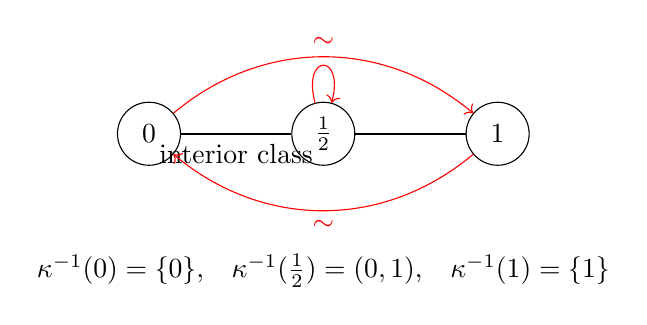
\begin{tikzpicture}[node distance=1.4cm]
  \node[circle,draw,minimum size=8mm] (z) {$0$};
  \node[circle,draw,minimum size=8mm,right=of z] (h) {$\half$};
  \node[circle,draw,minimum size=8mm,right=of h] (o) {$1$};
  \draw[thick] (z) -- node[below] {interior class} (h) -- (o);
  \draw[->,bend left=40,red] (z) to node[above] {$\negc$} (o);
  \draw[->,bend left=40,red] (o) to node[below] {$\negc$} (z);
  \draw[->,loop above,red] (h) to (h);
  \node[below=1.0cm of h,align=center] {$\collapse^{-1}(0)=\{0\}$,\quad
  $\collapse^{-1}(\half)=(0,1)$,\quad
  $\collapse^{-1}(1)=\{1\}$};
\end{tikzpicture}
\caption{The Kleene collapse keeps the two boundaries and identifies
all interior values.}
\label{fig:collapse}
\end{figure}

\begin{theorem}[Collapse homomorphism]
\label{thm:collapse}
For all $a,b\in[0,1]$,
\[
  \collapse(\negc a)=\negc\collapse(a),\qquad
  \collapse(a\conjc b)=\collapse(a)\wedge\collapse(b),\qquad
  \collapse(a\disjc b)=\collapse(a)\vee\collapse(b).
\]
\end{theorem}

\noindent
Lean: \Lean{Cred.collapse\_neg},
\Lean{Cred.collapse\_conj},
\Lean{Cred.collapse\_disj}.

This collapse is rigid.

\begin{theorem}[Three-element quotient]
\label{thm:three-quotient}
Any surjective map $\phi:[0,1]\to\three$ that preserves complement
and product sends $\half$ to $\half$ and, up to swapping $0$ and $1$,
sends the boundary values to the boundary values.  The Kleene quotient
is therefore the unique non-trivial three-element quotient of this
signature.
\end{theorem}

\noindent
Lean: \Lean{Cred.three\_element\_quotient\_unique}.

A sharper rigidity result holds if multiplication is allowed by
arbitrary real scalars rather than only by unit-interval values.

\begin{theorem}[No finite real-multiplicative quotient]
\label{thm:real-quotient}
No non-trivial finite quotient compatible with complement and
unrestricted real multiplication exists.
\end{theorem}

\noindent
Lean: \Lean{Cred.RealCongruence.no\_nontrivial\_finite\_quotient}.

The proof is a scaling argument.  A finite quotient makes powers of
$1/2$ cycle.  Unrestricted multiplication cancels the earlier power,
forcing $1\sim(1/2)^p$.  Complement then gives
$0\sim 1-(1/2)^p$, a positive value.  That collapses every value to
$0$.

\section{Consequence: Positivity and Certainty}

Let formulas be built from atoms using $\negc,\conjc,\disjc$.
For a valuation $v:\alpha\to[0,1]$, write $\val{\varphi}_v$ for
evaluation.

There are two natural designation thresholds:
\[
  \text{positive: }\val{\varphi}_v>0,\qquad
  \text{certain: }\val{\varphi}_v=1.
\]
LP designates $\half$ and $1$; K$_3$ designates only $1$.

\begin{theorem}[Formula bridge]
\label{thm:formula-bridge}
For every list of premises $\Gamma$ and conclusion $\varphi$:
\[
\Gamma\models_{\mathrm{LP}}\varphi
\quad\Longleftrightarrow\quad
\forall v\,
\bigl((\forall\gamma\in\Gamma,\ \val{\gamma}_v>0)
\Rightarrow \val{\varphi}_v>0\bigr),
\]
and
\[
\Gamma\models_{\mathrm{K3}}\varphi
\quad\Longleftrightarrow\quad
\forall v\,
\bigl((\forall\gamma\in\Gamma,\ \val{\gamma}_v=1)
\Rightarrow \val{\varphi}_v=1\bigr).
\]
\end{theorem}

\noindent
Lean: \Lean{Cred.lp\_formula\_bridge},
\Lean{Cred.k3\_formula\_bridge}.

\begin{figure}[h]
\centering
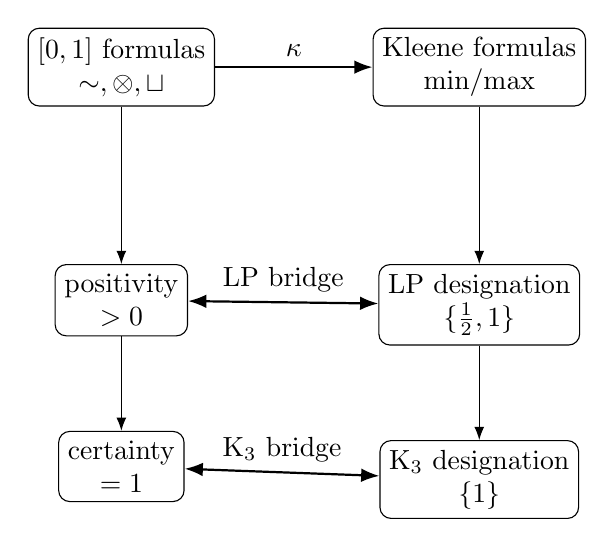
\begin{tikzpicture}[node distance=2.0cm,>=Latex]
  \node[draw,rounded corners,align=center] (r) {$[0,1]$ formulas\\
  $\negc,\conjc,\disjc$};
  \node[draw,rounded corners,align=center,right=of r] (k) {Kleene formulas\\
  min/max};
  \node[draw,rounded corners,align=center,below=of r] (p) {positivity\\
  $>0$};
  \node[draw,rounded corners,align=center,below=of k] (lp) {LP designation\\
  $\{\half,1\}$};
  \node[draw,rounded corners,align=center,below=1.2cm of p] (c) {certainty\\
  $=1$};
  \node[draw,rounded corners,align=center,below=1.2cm of lp] (k3) {K$_3$ designation\\
  $\{1\}$};
  \draw[->,thick] (r) -- node[above] {$\collapse$} (k);
  \draw[<->,thick] (p) -- node[above] {LP bridge} (lp);
  \draw[<->,thick] (c) -- node[above] {K$_3$ bridge} (k3);
  \draw[->] (r) -- (p);
  \draw[->] (k) -- (lp);
  \draw[->] (p) -- (c);
  \draw[->] (lp) -- (k3);
\end{tikzpicture}
\caption{The propositional bridge.  Collapse commutes with formula
evaluation, and the two designation policies become positivity and
certainty on the real interval.}
\label{fig:bridge}
\end{figure}

Classical logic is still present.  Restrict valuations to $\{0,1\}$.
Then positivity and certainty coincide with ordinary Boolean truth.
\begin{quote}\scriptsize
\begin{tabular}{@{}l@{}}
Lean anchors: \\
\Lean{Cred.crisp\_embedding}\\
\Lean{Cred.crisp\_certainty\_iff\_classical}\\
\Lean{Cred.crisp\_positivity\_iff\_classical}
\end{tabular}
\end{quote}

\section{Inference as Inverse-Image Inclusion}
\label{sec:inference-principle}

Conditioning and consequence are one construction.  Each fixes
constraints, forms the set of points those constraints admit, and
accepts a conclusion exactly when it holds across the whole set.

Fix the value object $([0,1],\conjc,\le)$ and read a threshold $t$ as
the up-set ${\uparrow}t=[t,1]$.  A \emph{constraint} on a point set $X$
is a pair $(f,S)$ with $f:X\to[0,1]$ and $S\subseteq[0,1]$; its
admissible set is the preimage $f^{-1}(S)$.  For a family $\Gamma$ of
constraints, $\mathrm{Mod}(\Gamma)=\bigcap_{(f,S)\in\Gamma}f^{-1}(S)$.
Inference is inclusion of admissible sets:
\[
\boxed{\;\Gamma\vdash(g,T)\quad:\Longleftrightarrow\quad
  \mathrm{Mod}(\Gamma)\subseteq g^{-1}(T).\;}
\]
This is the closure of the Galois connection between constraints and
points, the ordinary shape of semantic consequence.  Cred's two
inferences are its valuation-level and value-level instances, and the
two words are not synonyms.  A \emph{valuation} is a whole assignment of
values to the atoms, one possible world; a \emph{value} is a single
number.  Entailment ranges over worlds: it asks what holds in every
valuation that designates the premises.  Conditioning fixes the two
numbers $j$ and $e$ and ranges over the candidate values $c$ of one
conditional.  Same operator, different point space.
\begin{center}
\begin{tabular}{@{}llll@{}}
\toprule
 & points $X$ & evaluation $f$ & target $S$ \\
\midrule
consequence $\Gamma\models_t\varphi$ & valuations $v$ &
  $v\mapsto\val{\varphi}_v$ & ${\uparrow}t$ \\
conditioning $\Cond(j,e)$ & values $c\in[0,1]$ &
  $c\mapsto c\conjc e$ & $\{j\}$ \\
\bottomrule
\end{tabular}
\end{center}
For consequence the admissible set is
$\bigcap_{\gamma\in\Gamma}\val{\gamma}^{-1}({\uparrow}t)$ and the query
is $\val{\varphi}^{-1}({\uparrow}t)$; this is the formula bridge and
threshold consequence.  For conditioning the admissible set is the
fiber $m_e^{-1}(j)=\Cond(j,e)$ of the chain rule, and a threshold query
$c\ge t$ is warranted exactly when $\Cond(j,e)\subseteq{\uparrow}t$,
which is the robust and dependence-sensitive split below.  The value
carrier plays both roles: it is the codomain of every evaluation and,
for conditioning, the point set itself.

\begin{figure}[h]
\centering
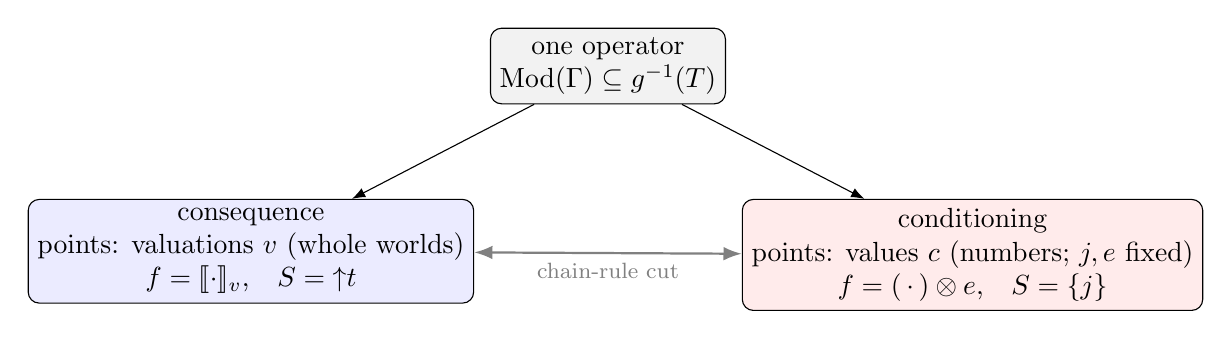
\begin{tikzpicture}[>=Latex]
  \node[draw,rounded corners,fill=gray!10,align=center] (op)
    {one operator\\$\mathrm{Mod}(\Gamma)\subseteq g^{-1}(T)$};
  \node[draw,rounded corners,fill=blue!8,align=center,
        below left=12mm and 2mm of op] (ent)
    {consequence\\points: valuations $v$ (whole worlds)\\$f=\val{\cdot}_v$,\quad $S={\uparrow}t$};
  \node[draw,rounded corners,fill=red!8,align=center,
        below right=12mm and 2mm of op] (con)
    {conditioning\\points: values $c$ (numbers; $j,e$ fixed)\\$f=(\,\cdot\,)\conjc e$,\quad $S=\{j\}$};
  \draw[->] (op) -- (ent);
  \draw[->] (op) -- (con);
  \draw[<->,thick,gray] (con) -- node[below,align=center,font=\footnotesize]
    {chain-rule cut} (ent);
\end{tikzpicture}
\caption{Two fibrations of one consequence operator.  Entailment runs
over valuations (whole worlds), conditioning over values (single
numbers); the chain-rule cut pushes a
value fiber forward into the valuation consequence, turning evidence
above $t$ and a conditional at least $\ell$ into a joint above
$\ell\conjc t$.}
\label{fig:two-fibrations}
\end{figure}

The three shapes of an admissible set are the same on both sides.  A
singleton forces one answer: positive evidence $c=j/e$, or premises
that pin the conclusion.  The full set forces nothing: zero evidence
gives $\Cond(0,0)=[0,1]$, and a glut leaves a surviving counter-valuation.
The empty set is incoherence: $j>e$ on the value side, no countermodel on
the valuation side, which is reductio.  No explosion is then not an extra
axiom.  Classical ex falso is the step ``the admissible set is empty,
therefore everything''; the principle declines it by reporting the empty
and full sets faithfully instead of collapsing either to anything.

One instance does not reduce to the other.  The conditioning evaluation
$m_e=(\,\cdot\,)\conjc e$ is a genuine map on values, but the next
section shows it does not descend to a connective on the collapsed
values: no truth function on $\{0,\half,1\}$ reproduces it.  The two
fibrations share a closure operator while the value fibration resists
internalization as an object-language conditional.  Unification at the
level of consequence; separation at the level of connectives.

\section{Why the Conditional Does Not Collapse}
\label{sec:no-cond-bridge}

Consequence is the inclusion $\mathrm{Mod}(\Gamma)\subseteq
\val{\varphi}^{-1}({\uparrow}t)$ of the previous section, and it
descends to the Kleene quotient.  Conditioning is the same inclusion on
the value fibration, and the next theorem shows it does \emph{not}
descend: the evaluation $m_e$ is no truth function on the collapsed
values.

\begin{theorem}[No truth-functional conditional bridge]
\label{thm:no-cond-bridge}
There is no function
$f:\three\times\three\to\three$ such that for every $a,b\in[0,1]$
with $b>0$,
\[
  \collapse\!\left(\frac{\min(a,b)}{b}\right)
  =f(\collapse(b),\collapse(a)).
\]
\end{theorem}

\noindent
Lean: \Lean{Cred.no\_truthfunctional\_cond\_bridge}.

\begin{proof}
Take $(a_1,b_1)=(0.3,0.7)$ and $(a_2,b_2)=(0.7,0.3)$.
All four inputs are interior, so
\[
  (\collapse(b_1),\collapse(a_1))
  =(\half,\half)
  =(\collapse(b_2),\collapse(a_2)).
\]
But
\[
  \collapse\!\left(\frac{\min(0.3,0.7)}{0.7}\right)
  =\collapse(3/7)=\half,
\]
while
\[
  \collapse\!\left(\frac{\min(0.7,0.3)}{0.3}\right)
  =\collapse(1)=1.
\]
Thus $f(\half,\half)$ would have to be both $\half$ and $1$.
\end{proof}

\begin{figure}[h]
\centering
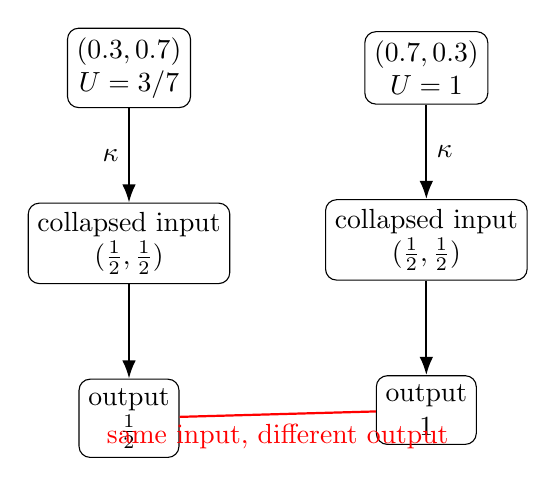
\begin{tikzpicture}[>=Latex,node distance=2.2cm]
  \node[draw,rounded corners,align=center] (a) {$(0.3,0.7)$\\
  $U=3/7$};
  \node[draw,rounded corners,align=center,right=of a] (b) {$(0.7,0.3)$\\
  $U=1$};
  \node[draw,rounded corners,align=center,below=1.2cm of a] (ca) {collapsed input\\
  $(\half,\half)$};
  \node[draw,rounded corners,align=center,below=1.2cm of b] (cb) {collapsed input\\
  $(\half,\half)$};
  \node[draw,rounded corners,align=center,below=1.2cm of ca] (oa) {output\\
  $\half$};
  \node[draw,rounded corners,align=center,below=1.2cm of cb] (ob) {output\\
  $1$};
  \draw[->,thick] (a) -- node[left] {$\collapse$} (ca);
  \draw[->,thick] (b) -- node[right] {$\collapse$} (cb);
  \draw[->,thick] (ca) -- (oa);
  \draw[->,thick] (cb) -- (ob);
  \draw[red,thick] (oa) -- node[below] {same input, different output} (ob);
\end{tikzpicture}
\caption{The obstruction to a truth-functional conditional on the
collapsed values.}
\label{fig:no-conditional}
\end{figure}

The obstruction is a small Lewis-style triviality result
\cite{lewis1976,vanfraassen1976,adams1975,mcgee1985}.  It differs
from the classical probability-of-conditionals problem in one respect:
the failure is visible in a finite quotient.  The quotient has thrown
away the ratio $a/b$, and no truth table can recover it.

The bridge does hold at boundaries:
\[
  a=0,\quad a=1,\quad b=1,\quad b\le a.
\]
Lean: \Lean{Cred.cond\_bridge\_boundary}.  These are exactly the
cases where the min-copula conditional lands on a boundary value or
where evidence is certain.

\section{Zero Evidence}

At zero evidence the chain rule is
\[
  c\cdot0=0.
\]
The equation holds for every $c$.  Three consequences share this one
root.

\begin{theorem}[Zero-evidence triple]
\label{thm:zero-triple}
The identity $c\cdot0=0$ yields:
\begin{enumerate}[label=(\roman*),nosep]
\item $\Cond(0,0)=[0,1]$;
\item LP explosion has a countermodel, witnessed by $\half$;
\item no collapsed truth function can recover the conditional value at
zero evidence.
\end{enumerate}
\end{theorem}

\noindent
Lean: \Lean{Cred.zero\_evidence\_duality},
\Lean{Cred.zero\_evidence\_duality\_cond}.

At zero evidence the constraint loses rank, and no value is selected.
Impossible evidence is not false evidence plus an implication rule.  One can add a convention after the fact, for example
``choose $1$'' or ``choose $\half$'', but the chain rule itself has no
reason to choose.

This locates the framework relative to imprecise probability
\cite{walley1991,troffaes2014,debock2015,wheeler2021}.  A set of
possible posteriors appears when the supplied constraint fails to
determine a point.  The set is not psychological indecision.  It is the
fiber of an equation.

Unknown dependence is a second source of a set, and it does not need
zero evidence.  Suppose the marginals $a,b$ are given but the joint is
not.  Coherence confines the joint to the Fr\'echet interval
$[\max(a+b-1,0),\,\min(a,b)]$, so for $b>0$ the admissible conditionals
are the image
\[
  \left\{\frac{j}{b}:\max(a+b-1,0)\le j\le\min(a,b)\right\}
  =\left[\frac{\max(a+b-1,0)}{b},\,\frac{\min(a,b)}{b}\right].
\]
A conclusion at a demanded threshold holds for every admissible joint
when this whole interval lies above the threshold, and is
dependence-sensitive when the interval straddles it.  The no-go theorem
of the previous section shows the collapse to $\three$ discards the
ratio $a/b$, so the order of work is fixed: carry the joint, or its
interval, check it against the threshold, and collapse only the
conclusions the quotient cannot distort.

\section{Self-Reference as Equations}

Let $\Phi:[0,1]\to[0,1]$.  A self-referential sentence governed by
$c=\Phi(c)$ has meaning
\[
  \Sol(\Phi)=\{c\in[0,1]:\Phi(c)=c\}.
\]

\begin{proposition}[Basic solution sets]
\label{prop:solution-sets}
\[
  \Sol(\negc)=\{\half\},\qquad
  \Sol(\mathrm{id})=[0,1],\qquad
  \Sol(\mathrm{id})=\Cond(0,0).
\]
\end{proposition}

\noindent
\begin{quote}\scriptsize
\begin{tabular}{@{}l@{}}
Lean anchors: \\
\Lean{Cred.Credence.solutions\_neg\_eq\_singleton}\\
\Lean{Cred.Credence.solutions\_id\_eq\_univ}\\
\Lean{Cred.Credence.truth\_teller\_same\_shape\_as\_zero\_evidence}
\end{tabular}
\end{quote}

The liar and the scalar Russell equation have the same form:
\[
  c=1-c.
\]
The unique solution is $c=\half$.  Classical logic sees no Boolean
solution.  The credence algebra sees one fixed point.

The truth-teller is
\[
  c=c.
\]
Every value solves it.  Its solution set is the same as zero-evidence
conditioning.  That is not a coincidence in the formal system: both
are unconstrained equations.

\section{Why the Conditional Must Stay External}

One might try to internalize conditioning as a binary connective
$a\Rightarrow b$.  Product logic does this by residuation
\cite{hajek1998,esteva2001,galatos2007}:
\[
  a\Rightarrow_{\Pi} b=
  \begin{cases}
    1, & a=0,\\
    \min(1,b/a), & a>0.
  \end{cases}
\]
This operation is forced by modus ponens plus conditional proof.
Let
\[
\begin{aligned}
\mathrm{MP}(f)&:\quad f(a,b)\conjc a\le b,\\
\mathrm{CP}(f)&:\quad c\conjc a\le b\Rightarrow c\le f(a,b),\\
\mathrm{Contraction}(f)&:\quad f(a,f(a,b))\le f(a,b).
\end{aligned}
\]

\begin{theorem}[Curry block]
\label{thm:curry-block}
No total function $f:[0,1]^2\to[0,1]$ satisfies
\[
  \mathrm{MP}(f)\ \wedge\ \mathrm{CP}(f)\ \wedge\
  \mathrm{Contraction}(f).
\]
\end{theorem}

\noindent
Lean: \Lean{Cred.Credence.curry\_block}.

\begin{proof}
MP and CP give full residuation.  Hence for $a>0$,
\[
  f(a,b)=\min(1,b/a).
\]
Choose $a=\half$ and $b=\quarter$.  Then
\[
  f(\half,\quarter)=\half,\qquad
  f(\half,f(\half,\quarter))=f(\half,\half)=1.
\]
Contraction would require $1\le\half$, contradiction.
\end{proof}

This explains the design decision.  The object language has negation,
conjunction, and disjunction.  Conditioning is a side judgment, a
constraint on supplied joint and evidence values.  Adding a total
internal conditional restores the very structural package that creates
Curry trouble.

\section{Threshold Consequence}

For $t\in[0,1]$, define
\[
  \Gamma\models_t\varphi
  \quad\Longleftrightarrow\quad
  \forall v\,
  \left(
  \forall\gamma\in\Gamma,\ t\le\val{\gamma}_v
  \right)
  \Rightarrow
  t\le\val{\varphi}_v.
\]
This consequence relation has reflexivity, monotonicity, and cut.
\begin{quote}\scriptsize
\begin{tabular}{@{}l@{}}
Lean anchors: \\
\Lean{Cred.threshold\_reflexivity}\\
\Lean{Cred.threshold\_monotonicity}\\
\Lean{Cred.threshold\_cut}
\end{tabular}
\end{quote}

Two thresholds are sharp:
\[
\text{explosion countermodel exists}
\quad\Longleftrightarrow\quad
0<t\le\half,
\]
and
\[
\text{excluded middle holds at threshold }t
\quad\Longleftrightarrow\quad
t\le\frac34.
\]
\begin{quote}\scriptsize
\begin{tabular}{@{}l@{}}
Lean anchors: \\
\Lean{Cred.threshold\_explosion\_countermodel\_iff}\\
\Lean{Cred.threshold\_excluded\_middle\_iff}
\end{tabular}
\end{quote}

\begin{figure}[h]
\centering
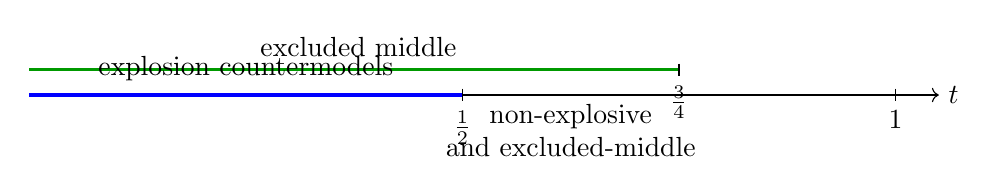
\begin{tikzpicture}[x=11cm,y=1cm]
  \draw[->] (0,0) -- (1.05,0) node[right] {$t$};
  \draw[very thick,blue] (0,0) -- (0.5,0);
  \draw[very thick,green!60!black] (0,0.32) -- (0.75,0.32);
  \draw (0.5,0.08) -- (0.5,-0.08) node[below] {$\half$};
  \draw (0.75,0.40) -- (0.75,0.24) node[below] {$\frac34$};
  \draw (1,0.08) -- (1,-0.08) node[below] {$1$};
  \node[above] at (0.25,0.05) {explosion countermodels};
  \node[above] at (0.38,0.37) {excluded middle};
  \node[align=center] at (0.625,-0.45) {non-explosive\\and excluded-middle};
\end{tikzpicture}
\caption{Sharp threshold facts.  For $\half<t\le 3/4$, explosion has
no threshold countermodel while excluded middle still holds.}
\label{fig:thresholds}
\end{figure}

The interval $\half<t\le3/4$ is the non-explosive band that still
validates excluded middle: contradiction licenses nothing, yet excluded
middle stays designated.  It is a status calculus for graded
consequence, not a foundation for mathematics.

\section{Toy Models and Worked Examples}
\label{sec:toy-models}

The architecture is finite and checkable.  Each subsection below is a
Lean example module with rational or Boolean data and concrete theorems.

\subsection{Pointwise truth is not connection}
Worlds $W=\{w_0,w_1,w_2,w_3\}$ carry Boolean propositions
$A,B,C:W\to\{0,1\}$.
\begin{center}
\begin{tabular}{@{}ccccc@{}}
\toprule
world & $A$ & $B$ & $C$ & $A\wedge B$\\
\midrule
$w_0$ & $1$ & $1$ & $1$ & $1$\\
$w_1$ & $1$ & $0$ & $1$ & $0$\\
$w_2$ & $0$ & $1$ & $1$ & $0$\\
$w_3$ & $0$ & $0$ & $1$ & $0$\\
\bottomrule
\end{tabular}
\end{center}
Entailment is truth-set inclusion,
$A\models B\iff\{w:A_w=1\}\subseteq\{w:B_w=1\}$
(\Lean{Cred.Examples.FiniteWorlds.entails\_iff\_subset}).
At $w_0$ all three are true, yet $A\not\models B$ because $w_1$ is a
countermodel (\Lean{Cred.Examples.FiniteWorlds.A\_not\_entails\_B}),
while $A\models C$
(\Lean{Cred.Examples.FiniteWorlds.A\_entails\_C}); pointwise agreement
does not fix the global relation
(\Lean{Cred.Examples.FiniteWorlds.pointwise\_does\_not\_determine}).
Dependence is invisible pointwise too.  The weightings
$\mu_1=(\tfrac14,\tfrac14,\tfrac14,\tfrac14)$ and
$\mu_2=(\tfrac12,0,0,\tfrac12)$ give equal marginals
$P(A)=P(B)=\tfrac12$ but different joints
$P(A\wedge B)=\tfrac14$ and $\tfrac12$
(\Lean{Cred.Examples.FiniteWorlds.joint\_not\_determined\_by\_marginals}).

\begin{figure}[h]
\centering
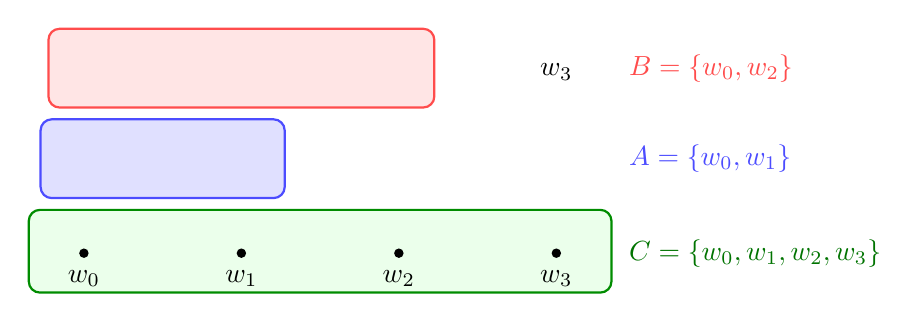
\begin{tikzpicture}[scale=1]
  \foreach \x/\name in {0/w_0, 2/w_1, 4/w_2, 6/w_3} {
    \node at (\x,2.3) {$\name$};
  }
  % C: all worlds
  \draw[rounded corners,draw=green!55!black,thick,fill=green!8]
    (-0.7,-0.5) rectangle (6.7,0.55);
  \node[green!45!black,anchor=west] at (6.8,0) {$C=\{w_0,w_1,w_2,w_3\}$};
  % A: w0,w1
  \draw[rounded corners,draw=blue!70,thick,fill=blue!12]
    (-0.55,0.7) rectangle (2.55,1.7);
  \node[blue!70,anchor=west] at (6.8,1.2) {$A=\{w_0,w_1\}$};
  % B: w0,w2
  \draw[rounded corners,draw=red!70,thick,fill=red!10]
    (-0.45,1.85) rectangle (4.45,2.85);
  \node[red!70,anchor=west] at (6.8,2.35) {$B=\{w_0,w_2\}$};
  \foreach \x/\name in {0/w_0, 2/w_1, 4/w_2, 6/w_3} {
    \fill (\x,0) circle (0.06);
    \node[below] at (\x,-0.1) {$\name$};
  }
\end{tikzpicture}
\caption{Truth sets in $W=\{w_0,\dots,w_3\}$ for $A=[1,1,0,0]$,
$B=[1,0,1,0]$, $C=[1,1,1,1]$.  $A\subseteq C$, so $A\models C$, but
$A\not\subseteq B$: world $w_1\in A\setminus B$ is the countermodel that
breaks $A\models B$ even though both hold at $w_0$.}
\label{fig:finite-worlds}
\end{figure}

\subsection{Robust conditioning from a Fr\'echet interval}
Take $a=\tfrac35$, $b=\tfrac{7}{10}$.  The joint is confined to
$[\tfrac{3}{10},\tfrac35]$
(\Lean{Cred.Examples.RobustConditioning.frechet\_lower},
\Lean{Cred.Examples.RobustConditioning.frechet\_upper}); the
independence joint is $\tfrac{21}{50}$
(\Lean{Cred.Examples.RobustConditioning.product\_joint}).  For $b>0$ the
admissible conditional ranges over the image interval
\[
  \left[\frac{3/10}{7/10},\,\frac{3/5}{7/10}\right]
  =\left[\tfrac37,\tfrac67\right]
\]
(\Lean{Cred.Examples.RobustConditioning.cond\_interval}; the general
image map is
\Lean{Cred.Dependence.cond\_interval\_of\_pos}).  The whole interval
clears the threshold $\tfrac13$, so that conclusion holds for every
admissible joint
(\Lean{Cred.Examples.RobustConditioning.robust\_at\_low\_threshold});
the threshold $\tfrac45$ lands inside the interval, so that conclusion
is dependence-sensitive
(\Lean{Cred.Examples.RobustConditioning.sensitive\_at\_high\_threshold}).
The three-valued summary of an interval is
\Lean{Cred.Dependence.collapseIntervalToThree}, returning a
\Lean{Cred.Dependence.RobustStatus} that records robustness or
sensitivity.

\begin{figure}[h]
\centering
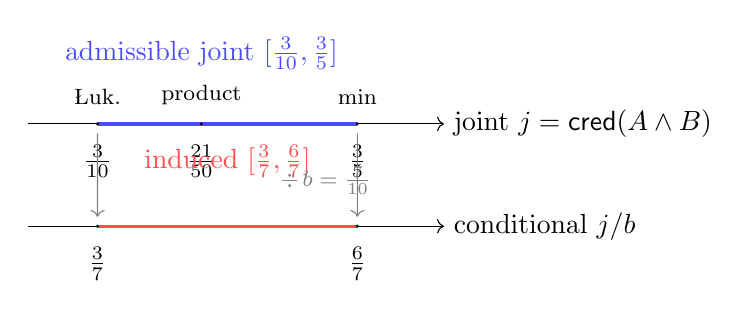
\begin{tikzpicture}[scale=1,x=11cm]
  % joint axis: from 0 to 1, but show the relevant window 0.25..0.65
  % map joint value j to x via x=j
  \def\jlo{0.3}   % 3/10
  \def\jprod{0.42} % 21/50
  \def\jhi{0.6}   % 3/5
  % joint number line
  \draw[->] (0.22,0) -- (0.7,0) node[right] {joint $j=\cred(A\wedge B)$};
  \draw[very thick,blue!70] (\jlo,0) -- (\jhi,0);
  \foreach \x in {\jlo,\jprod,\jhi} { \fill (\x,0) circle (0.6pt); }
  \node[below=4pt] at (\jlo,0) {$\tfrac{3}{10}$};
  \node[below=4pt] at (\jprod,0) {$\tfrac{21}{50}$};
  \node[below=4pt] at (\jhi,0) {$\tfrac{3}{5}$};
  \node[above=2pt,align=center] at (\jlo,0.05) {\footnotesize\L uk.};
  \node[above=2pt,align=center] at (\jprod,0.05) {\footnotesize product};
  \node[above=2pt,align=center] at (\jhi,0.05) {\footnotesize min};
  \node[blue!70,above=16pt] at (\jprod,0) {admissible joint $[\tfrac{3}{10},\tfrac35]$};
  % conditional axis below: cond = j/(7/10)
  \draw[->] (0.22,-1.3) -- (0.7,-1.3) node[right] {conditional $j/b$};
  \draw[very thick,red!70] ({3/7*0.7},-1.3) -- ({6/7*0.7},-1.3);
  \foreach \v in {3,6} { \fill ({\v/7*0.7},-1.3) circle (0.6pt); }
  \node[below=4pt] at ({3/7*0.7},-1.3) {$\tfrac{3}{7}$};
  \node[below=4pt] at ({6/7*0.7},-1.3) {$\tfrac{6}{7}$};
  \node[red!70,above=14pt] at ({4.5/7*0.7},-1.3) {induced $[\tfrac37,\tfrac67]$};
  % divide-by-b arrows
  \draw[->,gray] (\jlo,-0.12) -- ({3/7*0.7},-1.18);
  \draw[->,gray] (\jhi,-0.12) -- ({6/7*0.7},-1.18);
  \node[gray,right] at (0.5,-0.72) {\footnotesize $\div\,b=\tfrac{7}{10}$};
\end{tikzpicture}
\caption{Fr\'echet band and its induced conditional interval for
$a=\tfrac35$, $b=\tfrac{7}{10}$.  The joint is confined to
$[\tfrac{3}{10},\tfrac35]$ with the three named couplings as marked
points.  Dividing by $b$ maps the band onto the conditional interval
$[\tfrac37,\tfrac67]$.}
\label{fig:frechet-interval}
\end{figure}

\subsection{Fuzzy t-norms as fixed dependence policies}
A t-norm used as the joint is one coupling policy, not the general
joint.  With $a=\tfrac35$, $b=\tfrac{7}{10}$ the admissible joint ranges
over the Fr\'echet interval $[\tfrac{3}{10},\tfrac35]$; three named
t-norms pick three points of it.
\begin{center}
\begin{tabular}{@{}lccl@{}}
\toprule
policy (t-norm) & joint $j$ & conditional $j/b$ & dependence \\
\midrule
\L ukasiewicz $\max(a{+}b{-}1,0)$ & $\tfrac{3}{10}$ & $\tfrac37$ & minimal overlap \\
product $a\cdot b$ & $\tfrac{21}{50}$ & $\tfrac35=a$ & independence \\
minimum $\min(a,b)$ & $\tfrac35$ & $\tfrac67$ & maximum positive \\
\bottomrule
\end{tabular}
\end{center}
Lean fixes the three joint values:
\Lean{Cred.Examples.RobustConditioning.frechet\_lower} ($\tfrac{3}{10}$),
\Lean{Cred.Examples.RobustConditioning.product\_joint} ($\tfrac{21}{50}$),
\Lean{Cred.Examples.RobustConditioning.frechet\_upper} ($\tfrac35$).
Each is a valid coupling, and the product policy makes the evidence
irrelevant ($j/b=a$).  None is the general joint: the supplied
$j=\cred(A\wedge B)$ may be any point of $[\tfrac{3}{10},\tfrac35]$, and
only that supplied value fixes the conditional.

\subsection{Robust three-valued collapse}
An interval verdict collapses to a \Lean{Cred.Dependence.RobustStatus}
through \Lean{Cred.Dependence.collapseIntervalToThree}, which records
whether a conclusion survives every admissible joint.  Four worked
cases, with anchors in \texttt{Cred.Examples.RobustCollapse}:
\begin{center}
\begin{tabular}{@{}lll@{}}
\toprule
interval & verdict & anchor \\
\midrule
$[\tfrac12,\tfrac12]$ & robust half &
  \Lean{collapse\_interval\_interior\_robust\_half}\\
$[\tfrac37,\tfrac67]$ & dependence-sensitive &
  \Lean{collapse\_interval\_boundary\_sensitive}\\
$[0,1]$ & underdetermined &
  \Lean{zero\_evidence\_collapse\_underdetermined}\\
$[1,0]$ & incoherent &
  \Lean{empty\_fiber\_collapse\_incoherent}\\
\bottomrule
\end{tabular}
\end{center}
The collapse happens after the dependence reasoning, not before: a
ternary status is a summary of an interval of joints, never a place
where dependence is invented.

\subsection{Semantic entailment is not proof use}
A toy proof object carries named assumptions, and
\Lean{Cred.ProofTheory.usedAssumptions} extracts the set actually used;
soundness is \Lean{Cred.ProofTheory.provenance\_sound}.  A proof of the
valid formula $B\disjc\negc B$ uses no assumption
(\Lean{Cred.Examples.ProofProvenance.entails\_but\_unused}), even though
it is valid, so any premise entails it.  Which theorem depends on which is therefore a
proof-provenance question, not an entailment one.

\begin{figure}[h]
\centering
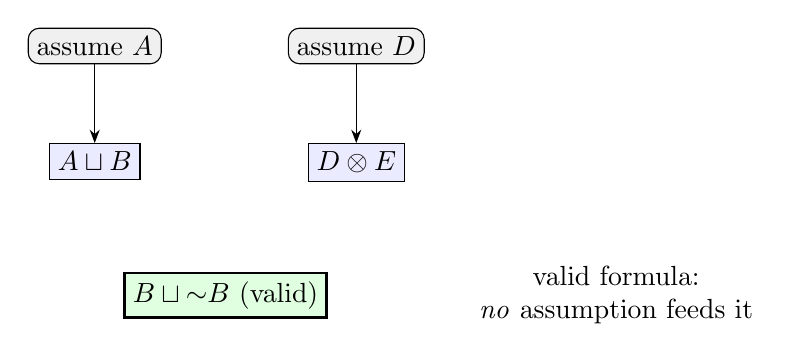
\begin{tikzpicture}[
    >=Stealth,node distance=10mm,
    pnasm/.style={draw,rounded corners,fill=gray!12,inner sep=3pt},
    pnstep/.style={draw,fill=blue!8,inner sep=3pt},
    pnconcl/.style={draw,thick,fill=green!12,inner sep=3pt}]
  \node[pnasm] (A) {assume $A$};
  \node[pnasm,right=16mm of A] (D) {assume $D$};
  \node[pnstep,below=of A] (s1) {$A\disjc B$};
  \node[pnstep,below=of D] (s2) {$D\conjc E$};
  \node[pnconcl,below=14mm of $(s1)!0.5!(s2)$] (g) {$B\disjc\negc B$ (valid)};
  \draw[->] (A) -- (s1);
  \draw[->] (D) -- (s2);
  % conclusion is valid: no edge into it from assumptions
  \node[align=center,right=18mm of g] {valid formula:\\ \emph{no} assumption feeds it};
\end{tikzpicture}
\caption{Proof-provenance DAG.  Edges record which nodes a derivation
actually consumes.  The assumptions $A,D$ feed their own consequences,
but the valid conclusion $B\disjc\negc B$ has no incoming edge: its
\Lean{Cred.ProofTheory.usedAssumptions} set is empty, so any premise
trivially entails it without being used.}
\label{fig:provenance-dag}
\end{figure}

\subsection{Local contradiction without explosion}
A branch whose assumptions contain both $A$ and $\negc A$ is locally
contradictory, yet the generative calculus, which has no explosion rule,
does not derive an unrelated atom $U$
(\Lean{Cred.Examples.Branches.local\_contradiction\_no\_explosion\_example};
the general statement is
\Lean{Cred.ProofTheory.local\_contradiction\_no\_explosion}).
This is the proof-theoretic image of $\Cond(0,0)=[0,1]$.

\subsection{The $\sqrt2$ dependency chain}
The number-theoretic core of the irrationality proof is a benchmark for
hypothetical branching.  From coprime $p,q$ with $p^2=2q^2$ and
$q\neq0$: $p$ is even
(\Lean{Cred.Math.sqrt2\_core\_even\_p}), hence $q$ is even
(\Lean{Cred.Math.sqrt2\_core\_even\_q}), contradicting coprimality
(\Lean{Cred.Math.not\_coprime\_if\_both\_even}); the chain closes at
\Lean{Cred.Examples.Sqrt2Branch.sqrt2\_core\_contradiction}.  The
recorded step list
\Lean{Cred.Examples.Sqrt2Branch.sqrt2\_dependency\_chain} localizes the
contradiction to the coprimality step: the false assumption is the
rational representation, and inconsistency enters at one named step
rather than spreading by explosion.

\begin{figure}[h]
\centering
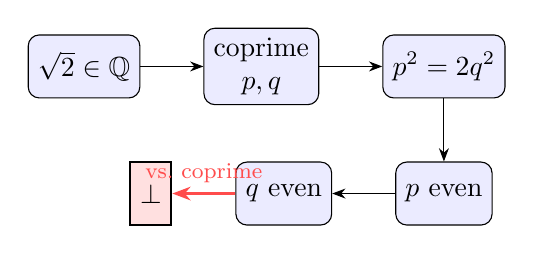
\begin{tikzpicture}[
    >=Stealth,
    nd/.style={draw,rounded corners,fill=blue!8,inner sep=3.5pt,
               minimum height=8mm,align=center},
    bad/.style={draw,thick,fill=red!12,inner sep=3.5pt,
                minimum height=8mm,align=center}]
  \node[nd] (r) {$\sqrt2\in\mathbb{Q}$};
  \node[nd,right=8mm of r] (c) {coprime\\$p,q$};
  \node[nd,right=8mm of c] (sq) {$p^2=2q^2$};
  \node[nd,below=8mm of sq] (pe) {$p$ even};
  \node[nd,left=8mm of pe] (qe) {$q$ even};
  \node[bad,left=8mm of qe] (bot) {$\bot$};
  \draw[->] (r) -- (c);
  \draw[->] (c) -- (sq);
  \draw[->] (sq) -- (pe);
  \draw[->] (pe) -- (qe);
  \draw[->,red!70,thick] (qe) -- node[above,font=\footnotesize,red!70]{vs.\ coprime} (bot);
\end{tikzpicture}
\caption{The $\sqrt2$ dependency chain.  Each node depends only on its
predecessor.  The contradiction enters at the single red step where
``$p,q$ both even'' meets the coprimality assumption; the false
assumption is the rational representation $\sqrt2\in\mathbb{Q}$ at the
head of the chain.}
\label{fig:sqrt2-chain}
\end{figure}

\section{Foundational Status}

The real interval is a semantic carrier, not an object-language
ontology.  Using $[0,1]\subset\Real$ supplies order, topology, and
multiplication for the model; the Boolean and three-valued fragments use
$\mathbf 2$ and the Kleene carrier.  The conditioning rule is the same
equation $c\conjc e=j$ on whichever carrier is chosen, and
$\Cond_V(j,e)$ is its fiber in the metatheory, not an object-language
set former.

\section{Proof Theory}

The proof layer has two judgment forms.  The scalar form proves
admissibility:
\[
  \Sigma\seq\Adm(c;j,e).
\]
The formula form proves labelled sequents:
\[
  \Gamma;\Sigma\seq_k\varphi,
\]
where $k$ is positive, certain, or a threshold $t$.

The scalar rules are deliberately small:
\[
\frac{\Adm(c;j,e)\in\Sigma}{\Sigma\seq\Adm(c;j,e)}
\quad
\frac{c\conjc e=j}{\Sigma\seq\Adm(c;j,e)}
\quad
\frac{}{\Sigma\seq\Adm(c;0,0)}
\]
and, for positive evidence,
\[
\frac{0<e\quad j\le e}{\Sigma\seq
  \Adm\!\left((j/e);j,e\right)}.
\]
Weakening and cut are structural:
\[
\frac{\Sigma\seq A\qquad A,\Sigma\seq B}{\Sigma\seq B}.
\]

Lean verifies scalar soundness and closed completeness:
\[
  \seq\Adm(c;j,e)
  \quad\Longleftrightarrow\quad
  c\in\Cond(j,e).
\]
It also verifies the boundary facts:
\[
  \seq\Adm(c;0,0)\quad\text{for every }c,
\]
and
\[
  0<e,\quad
  \seq\Adm(c_1;j,e),\quad
  \seq\Adm(c_2;j,e)
  \quad\Longrightarrow\quad
  c_1=c_2.
\]
\begin{quote}\scriptsize
\begin{tabular}{@{}l@{}}
Lean anchors: \\
\Lean{Cred.Credence.AdmDerivation.closed\_iff\_mem\_cond}\\
\Lean{Cred.Credence.zeroEvidence\_derivable}\\
\Lean{Cred.Credence.closed\_unique\_of\_pos}
\end{tabular}
\end{quote}

The formula calculus keeps conditioning external.  Its chain rule is a
cut between an admissibility side judgment and a formula bound:
\[
\frac{
  \Gamma;\Sigma\seq_t E
  \qquad
  \Sigma\seq\Adm(c;J,E)
  \qquad
  \ell\le c
}{
  \Gamma;\Sigma\seq_{\ell\conjc t} J
}.
\]
There is no rule introducing an implication formula $E\to J$.
Lean proves soundness for the labelled calculus and for kernel
certificates:
\[
  \Gamma;\Sigma\seq_k\varphi
  \quad\Longrightarrow\quad
  \text{every model of }\Gamma,\Sigma\text{ satisfies }k(\varphi).
\]
The cut-free fragment embeds into the full calculus, and cut is
semantically admissible.  Completeness holds for the closed threshold,
certainty, and positivity fragments because the corresponding semantic
consequence relation is available as a proof rule.  This is the exact
proof-theoretic status: sound external conditioning, no internal arrow,
and no ex-falso derivation.

\section{Relation to Existing Work}

\paragraph{Fuzzy and many-valued logic.}
Product logic uses the product t-norm and its residuum
\cite{hajek1998,esteva2001,cintula2011}.  Probabilistic fuzzy logics
and coherent conditional-probability logics also use many-valued
languages to reason about probability operators
\cite{hajek1995,flaminio2009,godo2006}.  More generally, fuzzy logics
choose a carrier and a conjunction-like operation, then study the
induced connectives.  The present system uses that algebraic data for
a different purpose.  It forms the external fiber
$\{c:c\conjc e=j\}$ and propagates that set when it is not a singleton.
It therefore does not identify conditioning with the product residuum.
The Curry block shows why: the full residuated package is incompatible
with contraction on this carrier.

\paragraph{Paraconsistent and three-valued logic.}
LP and K$_3$ arise through the collapse to
$\{0,\half,1\}$ \cite{kleene1952,asenjo1966,priest1979,belnap1977}.
The new claim is the exact formula-level bridge:
LP is positivity, K$_3$ is certainty.  The bridge is then shown to fail
for conditioning.

\paragraph{Connectives and consequence.}
Non-classical logic already separates an object-language conditional
from a metalanguage consequence relation \cite{priest2008,anderson1975}.
Classical logic can hide the distinction because $A\models B$ coincides
with validity of $A\supset B$.  That coincidence is not structural.  It
fails or changes in many non-classical settings.  Cred uses the
separation as a design rule: conditioning is the external judgment
$\Adm(c;j,e)$, not a new truth-functional connective.  The additional
claim is algebraic.  The external relation is fixed by $c\conjc e=j$,
and its zero-evidence fiber cannot be represented by any collapsed
truth function.

\paragraph{Conditionals.}
The de Finettian line studies trivalent truth conditions and their
proof theory \cite{egre2020part1,egre2021,egre2025}.  This paper takes
a different route.  It does not add a conditional truth table.  It
treats conditional credence as the admissibility relation determined
by the chain rule.

\paragraph{Probability and imprecision.}
Cox and Jaynes read probability as extended logic
\cite{cox1961,jaynes2003}.  Standard conditional probability uses
division at positive evidence, and H\'ajek gives reasons not to treat
that ratio as the whole concept \cite{hajek2003conditional}.  R\'enyi
and Popper instead take
conditional probability as primitive
\cite{renyi1955,popper1959,krauss1968,dubins1975}.  Disintegration and
Markov-kernel accounts condition by families of measures over fibers or
level sets \cite{chang1997,fritz2020}.  De Finetti-style conditional
events make the false-antecedent case void, and coherence theory studies
compounds of such conditionals
\cite{definetti1936,gilio2013,gilio2014,flaminio2020conditionals}.
Imprecise probability studies sets of probabilities as first-class
objects \cite{walley1991,troffaes2014}.  Natural and regular extension
handle lower-probability-zero updating, and full conditional
probabilities can force imprecision
\cite{debock2015,wheeler2021}.  These schools already supply most
ingredients: positive-evidence division, primitive conditionals,
conditioning over fibers, void antecedents, and set-valued updating.
The word ``fiber'' is therefore not new here.  Cred puts a smaller
invariant under these ingredients.  The set $\Cond(j,e)$ is the
preimage of one scalar equation.  It becomes wide exactly when evidence
is zero.  Its width records loss of constraint, not subjective
indecision.

\paragraph{Conditional-event algebras.}
Conditional-event algebras are richer object theories: they build
compound conditionals and probabilities over them.  Cred is narrower.
It keeps the scalar value, the supplied joint, and the admissible
fiber.  The same chain-rule fiber works on $[0,1]$, on the Boolean
carrier, and on three-valued variants.

\section{What Is Actually Novel}

The novelty is not the product t-norm, the Kleene lattice, primitive
conditional probability, conditioning along fibers, set-valued
probability, fuzzy probability logic, conditional-event algebra, or
paraconsistency.  Those are established.  The claim is the verified
conjunction of eight statements:
\[
\begin{array}{ll}
\text{(N1)} &
\Adm_V(c;j,e)\Longleftrightarrow c\conjc e=j
\text{ as a carrier-uniform fiber semantics};\\[1mm]
\text{(N2)} &
\text{propagation of non-singleton fibers, with }
\Cond(0,0)=[0,1]\text{ as no ex falso};\\[1mm]
\text{(N3)} & \text{LP/K$_3$ collapse bridges for full formulas};\\[1mm]
\text{(N4)} & \text{no truth-functional bridge for conditioning};\\[1mm]
\text{(N5)} & \text{scalar admissibility proof theory (sound, closed-complete},\\
  & \text{plus a generative connective fragment with direct soundness)};\\[1mm]
\text{(N6)} & \text{Curry block explaining why no internal arrow is added};\\[1mm]
\text{(N7)} & \text{value, dependence, and conditioning as separate inputs:}\\
  & \text{the joint is supplied, and unknown dependence propagates an interval};\\[1mm]
\text{(N8)} & \text{a first formalized cut of the foundation layers}\\
  & \text{(dependence contexts, robust collapse, provenance, branches).}
\end{array}
\]
Together they give a clean separation theorem in words:

\[
\boxed{
\text{truth-functional consequence can collapse;
conditional inference cannot.}}
\]

This is the submission line.  Adjacent material belongs in appendices
only if a referee asks for it, or in separate papers with different
venues.

\section{Toward a Foundation for Mathematics}
\label{sec:foundations}

The scalar kernel is not yet a foundation.  A foundation must keep four
structures separate: the value of a formula, semantic consequence over
all valuations, the supplied dependence (a joint or family of joints),
and proof provenance (which assumptions a derivation uses).  Ordinary
prose collapses these; the toy modules above formalize a first cut of
each missing layer.  The table records status against the Lean
development.

\begin{center}
\begin{tabular}{@{}p{0.27\linewidth}p{0.40\linewidth}p{0.27\linewidth}@{}}
\toprule
Layer & Formalized now (anchor) & Remaining \\
\midrule
Dependence contexts &
exact/coherent/interval contexts and joint families, with the
interval-to-fiber image (\Lean{Cred.Dependence}) &
credal networks over many propositions \\[2pt]
Robust collapse &
\Lean{Cred.Dependence.collapseIntervalToThree} into
\Lean{Cred.Dependence.RobustStatus} &
status-preserving rule propagation \\[2pt]
Proof provenance &
\Lean{Cred.ProofTheory.usedAssumptions},
\Lean{Cred.ProofTheory.provenance\_sound} &
full DAG over the foundation language \\[2pt]
Hypothetical branches &
\Lean{Cred.ProofTheory.local\_contradiction\_no\_explosion} &
$T+R$ over genuine theories \\[2pt]
Generative calculus &
local connective rules (conjunction introduction at threshold
$s\conjc t$ and elimination, disjunction introduction, double negation)
with \Lean{Cred.ProofTheory.generative\_sound}, no semantic-oracle rule &
quantifiers, equality, induction; syntactic completeness \\[2pt]
Mathematics seed &
parity, divisibility, the $\sqrt2$ core contradiction
(\Lean{Cred.Math}, \Lean{Cred.Examples.Sqrt2Branch}) &
full real-number development \\
\bottomrule
\end{tabular}
\end{center}

Two honesty markers.  The labelled calculus of the previous section is
sound and closed-complete because the semantic consequence relation is
admitted as a proof rule; that is an interface result, not a deep
syntactic completeness theorem.  The new generative fragment
(\Lean{Cred.ProofTheory.Generative}) removes the oracle rule for the
connective fragment and proves soundness directly, but it does not yet
cover quantifiers, equality, or induction.  Classical mathematics is
recovered at certainty on crisp structures; probability enters when the
joint context is supplied or learned; ternary and binary views are
robust summary layers, not places where dependence is invented.

\section{Lean Artifact}

All formal claims cited above are present in the current Lean
development under `lean/Cred`.  The core files are:
\[
\begin{array}{ll}
\text{values} & \Lean{Cred/Core/Value.lean},\\
\text{conditioning} & \Lean{Cred/Cond/Admissible.lean},\\
\text{admissibility proof theory} & \Lean{Cred/Cond/Proof.lean},\\
\text{collapse} & \Lean{Cred/Collapse/Hom.lean},\\
\text{LP/K$_3$ bridge} & \Lean{Cred/Bridge/LPK3.lean},\\
\text{conditional no-go} & \Lean{Cred/Bridge/CondBridge.lean},\\
\text{Curry block} & \Lean{Cred/Bridge/Curry.lean},\\
\text{labelled sequents} & \Lean{Cred/Sequent.lean},\\
\text{kernel certificates} & \Lean{Cred/Kernel.lean},\\
\text{cut and completeness} & \Lean{Cred/CutElim.lean}, \Lean{Cred/Completeness.lean},\\
\text{solution sets} & \Lean{Cred/Fixpoint.lean},\\
\text{thresholds} & \Lean{Cred/Threshold.lean},\\
\text{dependence contexts} & \Lean{Cred/Dependence/*.lean},\\
\text{generative calculus} & \Lean{Cred/ProofTheory/*.lean},\\
\text{toy models} & \Lean{Cred/Examples/*.lean}.
\end{array}
\]

The intended verification command is:
\[
  \texttt{cd lean \&\& lake build}.
\]
The manuscript itself is built by:
\begin{quote}\small\ttfamily
cd singlepaper\\
latexmk -pdf -interaction=nonstopmode -halt-on-error paper.tex
\end{quote}

\section{Conclusion}

The algebra is small:
\[
  \negc c=1-c,\qquad a\conjc b=ab,\qquad
  a\disjc b=a+b-ab,\qquad \Adm(c;j,e)\Longleftrightarrow ce=j.
\]
The lesson is also small.  A conditional is not a truth value waiting
to be tabulated.  It is a constraint that may determine one value,
many values, or none.  The set $\Cond(j,e)$ is the fiber of that
constraint, once the surrounding mathematics permits set notation.

At positive evidence, the chain rule recovers ordinary division.  At
zero evidence, it refuses to manufacture information.  The Kleene
collapse explains why positivity gives LP and certainty gives K$_3$.
The no-go theorem explains why conditioning does not extend to
that collapse.  The Curry block explains why the system should not add
an internal arrow to repair this.

The formal core is therefore not a new truth table.  Consequence and
conditioning are one inference, the inclusion of the admissible set the
constraints cut out; the separation is that only the value fibration
resists collapse to a truth-functional connective.

\bibliographystyle{alpha}
\bibliography{../cred,refs}

\end{document}
